\section{How the backends were built}\label{sec:process}

We carried out this work in a way that differs enough from how \galpy\
was developed before that we describe it in a section of its own.
Because an AI agent wrote the code, the question of how one comes to
trust such code is as much a part of this paper as the code itself. In
this section, we describe the organization of the work, how we reviewed
it, the stretch during which the agent worked without supervision, how
we made the existing test suite pass under the new backends, and the
checks through which we established that the code is correct. Because the division of labor between the human author and the
agent is the subject here, this section names them separately, as JB
and the agent.

\subsection{Organization}\label{sec:process-organization}

Work started on 2026 June 1 with a design discussion between JB and
Claude, Anthropic's AI coding agent, used through the \texttt{Claude
  Code} environment, which has access to a shell, to the \galpy\
repository, and to \github. The discussion settled the scope (all of
\galpy, on both \jax\ and \torch) and the constraints described in
\sectionname~\ref{sec:design}: byte-identity of the \numpy\ path, an
unchanged interface, no compilation inside \galpy, and the existing test
suite as one of the main acceptance tests. Passing the suite was not the
only goal: the coverage of the code by the tests was not to decrease
either (see the rules below). The first code, which took a day to
write, was a pilot that made two potentials run under all three array
libraries and checked value parity, gradients against finite
differences, and the identities between the potential, its forces, and
its second derivatives under automatic differentiation.

The work was organized in branches of the \galpy\ repository. \galpy's
main branch, from which version~1.x is released, continued to receive
its usual maintenance, as well as the fixes to the existing \numpy\ and
\cc\ code that the backend work turned up, which we always made there
first (\sectionname~\ref{sec:process-fixes}). The backend code was
developed on a long-lived \emph{backend branch}, to which every backend
change was proposed as a pull request (PR), either directly or through a
short-lived branch of its own when a change was split into several PRs.
The backend branch is periodically rebased onto the main branch, without
merge commits, so that it always contains the main branch's fixes, and it
becomes \galpy's version~2, released as pre-releases while the main branch
continues for now as version~1.x. The three-dimensional variational
equations had their own branch, which was merged into the main branch,
and during the stretch described in
\sectionname~\ref{sec:process-autonomous} the agent worked on a separate
development branch.

Between 2026 June 1 and October 30, 723 PRs were opened for this work,
of which 696 were merged: 602 on the backend branch and its sub-branches,
29 for the three-dimensional variational equations, and 65 against
\galpy's main branch, of which 40 fixed defects in the existing \numpy\
and \cc\ code that the backend work had found
(\sectionname~\ref{sec:process-fixes}), 16 added capabilities or
speed-ups to that code that came out of the work, and 9 concerned the
tests and the continuous integration. The merged PRs have a median size
of 182 changed lines (quartiles 74 and 372 lines).
We kept the size small on purpose, because a PR is reviewable when it
does one thing, and a backend migration of one module, with its tests,
is one thing. We split larger pieces of work into stacks of dependent
PRs that are reviewed in order (101 of the PRs are members of such stacks);
for example, we split the migration of the spherical DFs by DF family
into a base PR and four PRs that each port one family, and the port of
the one-dimensional inverse action--angle code into three. Each PR
carries a description of what was changed, the measurements that
support it (timings, parity counts, gradient errors), and what was
explicitly left out, such that the description can be reviewed without
re-deriving it from the diff.

The rate of PRs varied with the kind of work: in June, 88 backend PRs
and 29 PRs for the three-dimensional variational equations were opened
as the agent migrated the potentials family by family, in parallel, from
a fixed template. July was the peak, with 176 backend PRs: the agent ported the orbit,
action--angle, and DF modules, the autonomous stretch started, and the PRs were small, one problem each. In August (114) and
September (112), the work turned to the compiled modes, the test ledger
of \sectionname~\ref{sec:process-ledger}, and
the harder DFs, with PRs that were fewer and larger, because the
remaining problems were coupled; October, the last month of the
work, added 135 through the 30th.
Over the same months, the repository received a separate stream of 58
PRs in August and September for another \galpy\ project, which shared
the continuous integration and matters for the costs below.

In round numbers, the work cost the following. The agent ran on a
fixed-price subscription to Anthropic's Claude: until 2026 June 25 the
``Max'' plan at its 20$\times$ tier, which Anthropic provided free of
charge, afterwards the 5$\times$ tier at about CAD~140 per month, and
for the final two weeks the 20$\times$ tier again.
Successive versions of the Claude Opus models did the coding, while
Claude Fable was used only to draft this paper and its major revisions.
The far larger cost was
the continuous integration, because every backend PR runs \galpy's test
suite in five modes over 22 shards, about 150 jobs of 20 to 90 minutes
each; the GitHub Actions bill for the repository at list price was
\$13,100 in June, \$16,500 in July, \$15,800 in August,
\$10,200 in September, and \$8,600 in October 2026. June,
July, and October were almost entirely this project; in August and
September the backend PRs were about three quarters of the PRs and, since a PR to
the main branch runs only the \numpy\ suite, a larger fraction of the
compute, such that about \$59,000 of the total is attributable to the
backend project. GitHub's Education program covered
this cost, which would otherwise have been prohibitive. The continuous
integration was crucial to establishing that the PRs were correct: it
ran every test in every mode on every PR, and it often turned up errors
that the local runs before pushing had not, in modes, shards, or
versions of the dependencies that the agent had not tried. It was also
the bottleneck of the project, because a PR could not be merged
before its matrix had run, the shards queued behind each other when
several PRs were open, and a flaky job meant a two-hour wait. We made
several of the engineering decisions---cancelling the runs
of superseded commits, running the compiled modes only on demand until
they were stable, running the touched tests under forced backends
locally before pushing---to spend less time in that queue. \github's
support for stacks of dependent PRs, which rebases the members of a
stack and retargets them as the lower ones merge, arrived only on 2026
July 30. Before then, we based dependent PRs on each other's branches by
hand, and several open PRs that touched the same files had to be rebased
onto each other by hand every time one of them changed or merged, each
rebase triggering a new run of the whole matrix; the stacks removed most
of that work.

JB fixed a few rules early and enforced them throughout. The \numpy\ path
had to remain byte-identical, and any deviation (\sectionname~\ref{sec:design-principles}
lists them) was flagged in the PR rather than absorbed.
The \jax\ and \torch\ paths had to pass the same tests at the same
tolerances; a tolerance could be loosened only for one test, only
slightly, and with a justification in the PR. Test coverage was not
allowed to decrease, not by a single line; in the end, the backend
branch leaves 14 of its 56,950 executable statements uncovered, against
24 of 41,704 on the main branch. Tests had to make meaningful assertions
at tight tolerances: values had to match their reference to a relative
$10^{-13}$ or better, often $10^{-14}$, and derivatives a finite
difference that is shown to converge; a test could never merely check
that a result is finite, and only tests of sampling had looser
tolerances, set by their Monte Carlo noise. A test that
passes under a backend only because the code silently fell back to
\numpy\ does not count, and the agent hunted down such \emph{numpy
islands} specifically (\sectionname~\ref{sec:process-islands}). Before
pushing any PR, the agent ran its tests locally under forced \jax\ and
\torch\ backends, which the \numpy-only checks cannot do, and measured
the \numpy\ byte-identity by comparing checksums of outputs between two
checkouts that differ only in the files of the PR.

\subsection{Review}\label{sec:process-review}

Every PR was reviewed before it was merged into the backend branch, and
JB merged all of them except during the stretch described in
\sectionname~\ref{sec:process-autonomous}, whose work JB reviewed before
it was merged into the backend branch. Much of the review was
conversational, in the session in which the agent worked, and
concerned design as much as code: that a hand-rolled root finder
belongs in a utility module or should be replaced by \scipy's, that
speed-ups are to be demonstrated by timing both versions rather than
asserted, that tests should go through public methods rather than
internal functions, and so on. Reviews on \github\ itself caught the
kinds of problems that reviews of human code catch: a variable omitted
from an OpenMP \texttt{private} clause, a coverage drop of one line that
the automated check had passed.

Claude Code records every message of a session, and the token counts of
every response, in a transcript, from which we can estimate how much
input the work took. This is an estimate, not an exact count, because
separating JB's own text from the material that he passed on (reports
from other agents, reviews, logs) relies on simple heuristics. Between
2026 June 4 and October 30, JB sent about 2,500 messages, on 141 of the
149 days, almost a quarter of them while the agent was working, which
then folded them into the task at hand. Most were short, with a median
length of 14 words, and in total they contain about 57,000 words of
JB's own text, or roughly 110 single-spaced pages, plus about 33,000
words that he passed on. Over the same period, the agent produced about
114 million output tokens (including its reasoning and its tool calls;
a third of them in subagents that it started) and read about 44 billion
input tokens, almost all of them its own context re-read from a cache at
every step; these numbers do not include the other agents whose reports
JB passed on. Review on \github\ itself was light by comparison: of the
494 PRs that the agent opened under its own account (from July 26 on),
JB left a formal review on 23 and comments on 24.

JB also used two other forms of review. First, at several points he ran
an independent AI code reviewer (OpenAI's Codex) over the agent's work and
passed its findings to the agent to address, usually by pasting them into
the conversation (18 reviews in all). These reviews
found real defects: a gradient of the incomplete gamma function that
was \texttt{nan} at the endpoint $x=0$ although its value was correct;
a quadrature routine documented as accepting arrays that was correct
only for scalars; a surface-density routine that used the backend
quadrature only when the height above the plane was traced, such that a
derivative with respect to the radius at fixed height fell back to
\scipy\ and failed; and a branch-selection rule in the compiled path of
the hypergeometric function that returned infinity where the eager path
was correct. The agent reproduced each finding before fixing it and
dropped the findings that it could not reproduce with a note saying why.
Second, before merging complex PRs, JB instructed the agent to run
adversarial reviews of its own work by independent agents whose only
task was to break the PR against the real code; these found, for
example, that a stream sampler handed the same random key to the
position- and velocity-angle samplers, and that the parity tests of an
early PR compared at a tolerance four orders of magnitude too loose to
catch the $10^{-16}$ differences from re-associated arithmetic. The
latter finding set the pattern for all subsequent work: the original
\numpy\ expression is kept byte-for-byte and only the branching is
rewritten, never an algebraically equivalent form.

\subsection{The autonomous stretch}\label{sec:process-autonomous}

From 2026 July 26 to August 9, JB was away on vacation and the agent worked on its
own, with the goal of making the whole existing test suite pass under
compilation and of emptying the ledger of expected failures. For this,
the agent opened PRs against a separate development branch, which it
merged itself once the continuous integration was green, under the
understanding that JB would review the accumulated branch on his return.
It could not merge into the backend branch or into \galpy's main
branch, and it could not change the continuous-integration
configuration. These were hard guardrails rather than instructions: the
agent worked through its own \github\ account, which was set up for this
purpose and whose access token lacks the permission to modify the
workflow files that define the continuous integration, and branch
rulesets on \github\ allow changes to the main and backend branches only
through PRs that pass the required checks and, for the duration of the
stretch, blocked all updates of these two branches. A scheduler woke the agent at regular intervals to ensure
that it kept going, and the agent kept a dated log of what it did and
why; this log, which runs to 60,000 lines for the summer, is part of the
repository that accompanies this paper.

In the two unsupervised weeks, the agent merged 74 PRs. JB was pleased
enough with the progress on his return that he let the unsupervised
procedure continue for a few more weeks, alongside his supervised work,
and 145 PRs in total went through the development branch before it was
merged into the backend branch on 2026 September 2, after JB had
reviewed it as a whole and with the help of a Codex review (the
latter's verdict, that ``the work is coherent, the ledger is honest,''
matched JB's own). The stretch
made clear both what such an agent can and cannot do. It burned the
compiled-mode ledger down from 100 to 15 failing tests in three days,
found and fixed a performance problem in the coercion of inputs that had
cost 178\,$\mu$s per call, resolved the interaction between
\astropy\ units and compilation, and found two pre-existing bugs in
\galpy's \numpy\ code that it validated against a 30-digit reference
before filing them as issues. It also introduced regressions, all of
which it found itself within days using the tools it had built for the
purpose---a traced sweep of the suite, a comparison of test durations
between runs---and fixed before JB returned; it misread a stale rule;
it once left conflict markers in a working tree, the type of error that
a human review would have spotted easily; and its summary table
of PRs fell out of date and had to be rebuilt from \github. The
scorecard that it wrote for itself judged the stretch against its goal
honestly: the ledger went from 392 to 140 entries against a target of
zero. We have kept this account in the paper because it is the kind of
information that a reader deciding whether to work this way needs. On
the whole, the autonomous stretch succeeded in keeping the agent working
productively while JB was away, but it did so because the agent had a
clear, limited, and verifiable goal---emptying the ledger---and work
towards the broader aims of the project, which require judgment about
what to build and how, would have been much harder to leave unsupervised.

\subsection{Making the test suite pass under every backend}\label{sec:process-ledger}

One of the main acceptance tests for the backends was \galpy's own test
suite, run under \numpy, under \jax\ and \torch\ in eager mode, and
under \jax\ and \torch\ with compilation at every entry point, for a
total of five modes. Leaving aside the 27 tests of the out-of-scope
torus-mapping code (below), the suite grew from 2,462 to 4,462 tests
over the course of this work, mainly because we split existing tests
up: tests that looped over all of \galpy's potentials inside a single
test, for example, became one test per potential, such that each
failure and success could be traced to its potential. We did not delete
or modify tests that failed under a backend, but listed them in a
\emph{ledger}, one line per test and mode, that marked them as expected
failures, such that the size of the ledger was the measure of what
remained to be done. A second ledger listed tests that passed under a
backend but exceeded the time limit that we set for a single test in
the continuous integration, 300\,s, which keeps one hung or pathologically
slow test from stalling a shard of the matrix, and a third lists the
tests of code that is permanently out of scope. We regenerated the
ledgers from the actual test results on demand, such that they could
not drift from reality, and the continuous integration posted a report
of each PR's results per file and mode, ledgered failures included, to
the PR, such that a reviewer saw at a glance what a PR fixed or broke.
In addition, we ran a dedicated set of tests of the backend code itself,
now 18,807 tests in 100 files.

\begin{figure*}[t!]
  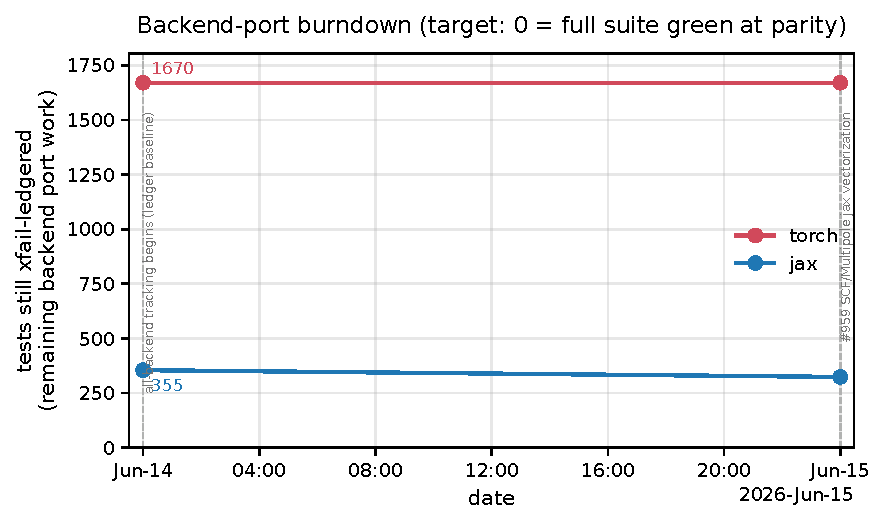
\includegraphics[width=\textwidth,clip=]{../figures/g13_ledger_burndown/g13_ledger_burndown.pdf}
  \caption{Tests of \galpy's existing test suite that pass under each
    backend, as a function of time, leaving aside the 27 tests of the
    out-of-scope torus-mapping code. The grey line is the size of the
    suite, which grows from 2,462 to 4,462 tests over the period (most
    of the jump on June 19 comes from splitting the potential tests into
    one test per potential); the colored curves show the number of these
    tests that pass under \torch\ (top) and \jax\ (middle) in eager mode
    (solid) and under compilation (dashed), that is, the size of the suite
    minus the tests that are ledgered as expected failures or as too slow,
    or skipped, under that mode, which is the shaded band. The compiled
    mode's ledgers are counted with the rules that the test configuration
    applied at each date; in August, \jax\ passes more tests under
    compilation than in eager mode because slow orbit tests that are
    skipped in eager mode run in reasonable time when compiled. The bottom
    panel shows the number of tests in the dedicated backend test
    modules; its jump in October is the two sweeps of
    \sectionname~\ref{sec:process-correctness}, which add 7,045
    parametrized cases. At the end, all 4,462 tests pass in every
    mode.}\label{fig:ledger}
\end{figure*}

\figurename~\ref{fig:ledger} displays how we brought the suite to pass.
On 2026 June 14, when the all-backend continuous integration was first
run, 1,042 tests failed under \jax\ and, a week later, 2,080 under
\torch; the difference between the two is almost entirely due to
\torch's rejection of \python\ scalars where \jax\ accepts them, and it
disappeared when we centralized the coercion of inputs (see
\sectionname~\ref{sec:design}). The eager ledgers were essentially empty
by 2026 September 12, and we emptied the compiled-mode ledgers, which
started at 100 and 146 tests when we introduced those modes, over the
following month. At the time of writing, the ledgers are empty in every
mode. The 27 tests of the torus-mapping code, which as a wrapper of an
external code is out of scope, are not run under the backends: the 23
tests of its own test module and four tests of the stream DF that build
the stream's track with it.
A ledger entry that covers a whole file hides how many tests it
contains, and the figure therefore counts the tests that each entry
matches at the time; early entries of this kind understated the \jax\
ledger by about 700 tests.

\subsection{How much of the suite runs on the backend}\label{sec:process-islands}

A test that passes under a forced backend shows that the code returned
the right answer, not that the backend computed it: a code path that
converts its input to \numpy, computes with \numpy\ or \scipy, and
converts the result back passes every check of a value. In the first
months, such \emph{numpy islands} were common, because the natural way
to add a backend path to a function, a branch on whether its input is a
backend array, at first took the \numpy\ branch for the \numpy\ inputs
of the existing tests even under a forced backend; a first backend version of
the action--angle code passed its tests under \jax\ in this way and was
rejected in review. Three mechanisms make the forced mode meaningful.
Functions branch on the resolved namespace rather than on the type of
their input, and the public entry points coerce their inputs to the
forced backend (\sectionname~\ref{sec:design-choosing}). Objects that
are constructed under a forced backend hold their parameters as backend
arrays, such that their methods compute on the backend also when they
are called from code that still uses \numpy. And on a GPU, an implicit
conversion of a device array to \numpy\ raises an error rather than
copying silently, such that running the suite on a GPU turns every
remaining implicit conversion into a test failure
(\sectionname~\ref{sec:design-gpu}).

To measure what remains, we instrumented a run of the existing suite
under forced \torch\ to record every place where \galpy\ hands backend
data to \numpy: implicit conversions by \numpy\ and \scipy,
explicit copies to the host, and regions in which \galpy\ deliberately
computes with \numpy.\footnote{We use \torch\ for this measurement,
  because \numpy\ reads a \jax\ array on the CPU through the buffer
  protocol, which bypasses the conversion method that the instrument
  intercepts.} We classified every such place by the reason for the
hand-off and every test by the least benign of its reasons
(\tablename~\ref{tab:islands}). Four reasons concern work that has to
happen on the host: \galpy's \cc\ extensions, for orbit integration and
the St\"{a}ckel actions, whose derivatives come from the state-transition
matrix and from custom derivative rules
(\sectionname~\ref{sec:orbit-paths}); decisions that need a value on the
host, such as a tolerance, a root bracket, the number of integration
steps, or a cache key; output to \astropy\ quantities or plots; and
\numpy\ functions that the test itself supplies, such as the density of
an expansion. Three are \numpy\ computations that could run on the
backend but have no reason to: constant tables built at construction
from parameters that are not differentiated, such as the spline of the
guiding radius or the coefficients of an expansion (a differentiated
parameter takes a backend path, as the sweep of
\sectionname~\ref{sec:process-correctness} verifies); sampling with
\numpy's global random-number generator, which the tests seed (a
backend random key runs the backend sampler); and the \python\
integrators of the \numpy\ code, which warn that their result is not
differentiable. The last is one documented exception that keeps
\numpy\ for \numpy\ inputs under a forced backend, while a backend input
or a differentiated parameter takes the backend path: a stream that the
tests build with \numpy\ before the backend is forced, whose lazily
computed track stays in \numpy\ like the stream itself.

\begin{table}
  \caption{Tests of the existing suite by how they hand backend data to
    \numpy\ under a forced \torch\ backend (4,353 tests that ran;
    cumulative).}\label{tab:islands}
  \centering
  \small
  \begin{tabular}{lrr}
    \hline
    hand-offs to \numpy\ at most & tests & share \\
    \hline
    none & 2,011 & $46.2\,\%$ \\
    + \galpy's \cc\ extensions & 2,321 & $53.3\,\%$ \\
    + decisions on the host & 3,153 & $72.4\,\%$ \\
    + output (units, plots) & 3,322 & $76.3\,\%$ \\
    + \numpy\ functions of the test & 3,389 & $77.9\,\%$ \\
    + constant tables & 3,949 & $90.7\,\%$ \\
    + \numpy's random numbers & 4,098 & $94.1\,\%$ \\
    + the \python\ integrators & 4,349 & $99.9\,\%$ \\
    + one documented exception & 4,353 & $100.0\,\%$ \\
    \hline
  \end{tabular}
\end{table}

When we first ran the instrument, 220 tests ($5.3\,\%$) passed through a
genuine island, \numpy\ computation that could and should run on the
backend: the transformation of an integrated orbit in the isochrone
approximation (55 tests), the \numpy\ track tables of
\texttt{streamdf} (53), the profiles of the disk DFs (39), \scipy\ root
finding for orbit quantities such as the guiding radius and for the
Lindblad resonances (49), and smaller sites in about 25 other functions,
among them the \texttt{MovingObjectPotential} (4 tests). We moved all of
these to the backend, in eight PRs, mostly with backend code that
already existed; the root finders, which now run on the backend also
for plain scalars under a forced backend, needed a bracketing that
evaluates the function at many points of the bracket at once, because
the 45 sequential evaluations of a bisection each cost a full eager
dispatch. The same instrumented run now finds no test that passes
through a genuine island (\tablename~\ref{tab:islands}): $46\,\%$ of the
tests never hand backend data to \numpy, $78\,\%$ do so only for work
that has to happen on the host, and the remaining $22\,\%$ use \numpy\
only for constant tables, for sampling with \numpy's random-number
generator, in the \python\ integrators, or in the one documented
exception.

\subsection{Fixes to \lowercase{\galpy}}\label{sec:process-fixes}

Running the same calculations through a second implementation, and
differentiating them, is an effective way to find bugs in the first, and
the backend work led to the 40 PRs against the main branch that fixed
\galpy's \numpy\ and \cc\ code (\sectionname~\ref{sec:process-organization}). The three-dimensional
variational equations, which require correct second derivatives of the
potential, found some of these: four potentials had incorrect
planar second derivatives in \cc, and the \cc\ second derivatives of
the basis-function potentials had the wrong sign in one component,
which the usual check that the determinant of the state-transition
matrix is one cannot catch. The comparison of the backend quadratures
with the existing ones found others: the plain Gauss--Legendre
quadrature of the action integrands in the adiabatic and St\"{a}ckel
approximations loses about four digits at the turning points, because
the integrands have square-root endpoints, and we regularized it; the
default absolute tolerance of \scipy's adaptive quadrature truncated
several small integrals (the outer tail of the Jeans velocity
dispersion, the surface density far from the plane); and the \cc\ and
\python\ implementations of the Chandrasekhar dynamical-friction force
interpolated the velocity dispersion with different splines, which
differed by a few parts in a thousand at small radii. The figures of
this paper, which we regenerate from scratch against the current code,
found yet others: the inverse-cumulative sampling of the
spherical DFs biased the sampled velocity dispersion low by about
$0.7\,\%$ at the default grid resolution, and the forces of the two-power
density profiles were off by up to $10^{-3}$ near the inner power-law
index of three. We fixed pre-existing defects of this kind in their
own PRs against the main branch, never quietly in the backend branch,
such that each is documented and their count is known.

\subsection{Establishing correctness}\label{sec:process-correctness}

JB does not take the code to be correct because an agent reports that
its tests pass; the reasons to believe that it is correct are the
following, roughly in order of weight. The \numpy\ path is byte-identical to the previous
version, measured by checksums of tens of thousands of output values per
PR, such that the entire body of validation that \galpy\ has accumulated
over more than a decade carries over. The backend paths pass the same tests at the
same tolerances, in five modes, and the only tests that do not run
under the backends are the 27 of the out-of-scope torus-mapping code
(\sectionname~\ref{sec:process-ledger}). We compared every derivative that the code can compute with a
finite difference whose convergence with step size is demonstrated
rather than assumed, or with an independent reference where one
exists: the derivatives of orbits with respect to their initial
conditions are computed by the variational equations in \cc\ and by
reverse-mode automatic differentiation through two different ODE
solvers, and the three agree
with each other and with finite differences of independently integrated
orbits to a few parts in $10^{10}$ (\figurename~\ref{fig:icjacobian}).
That no derivative was missed is checked by a sweep: for every public
potential, action--angle, and distribution-function class and the
stream-impulse functions, it differentiates each numeric parameter and
one input coordinate, 761 derivatives in 199 configurations, under
compiled \jax\ and eager \torch, with the inputs given as backend
arrays, as \python\ floats, and under a forced backend, and compares
them with converged finite differences of the \numpy\ code. When we
first ran it, about 60 combinations of class and parameter raised an
error or worked only eagerly, and nine families of derivatives were
silently wrong, zero, or disconnected from the parameter; for example,
\torch\ orbit integration with \galpy's \cc\ integrators dropped the
derivatives with respect to the potential's parameters, which made those
of a stream model wrong by up to a factor of 45. We fixed all of them,
and the sweep, 2,791 cases, now runs in the continuous integration. The
one remaining exception is by design: under compilation, the anisotropy
of a constant-anisotropy distribution function cannot be traced, because
it selects the order of a derivative in the inversion. A second sweep
gives each parameter and input coordinate in turn as a concrete backend
array that is not differentiated, and checks that every output comes
back on that backend with the \numpy\ values (4,249 cases); when we
first ran it, about 1,200 cases returned \numpy\ arrays, raised an
error, or returned an array of the wrong shape, and all of them now
pass.
Where the backend code implements a numerical method of its own---a
special function, a quadrature, a root finder---we checked it against
\scipy\ and against \texttt{mpmath} at 30 to 50 digits and validated the
reference itself before use, because the analytic formula one reaches
for first is sometimes the one that is wrong. JB, a second AI system,
and adversarial agents reviewed the code, and running it on two GPUs,
which the continuous integration cannot do, found the device-placement
bugs that are invisible on a CPU. And
the figures of this paper, each of which is produced by a script that is
re-run against the current code and whose output is checked against a
stored hash, found several of the bugs listed above. None of these
checks is sufficient on its own, and JB would not have accepted the code
on the basis of any one of them, only on their combination together with
his own review of the code itself.
